% Text Parse Tree Example
%
% File:         text-parse-tree.tex
% Author:       Bob Walton (walton@acm.org)
% Date:      	Sat Jan 12 08:48:09 EST 2013
  
\documentclass{minimal}
\usepackage[paperheight=2in,paperwidth=2in,
            height=2in,hoffset=0.05in,
	    voffset=0.05in,left=0in,width=2in]{geometry}
\usepackage{color}
\usepackage[usenames]{xcolor}
\usepackage{tikz}
\usepackage{scalefnt}
\usetikzlibrary{arrows}
\begin{document}
\raggedright
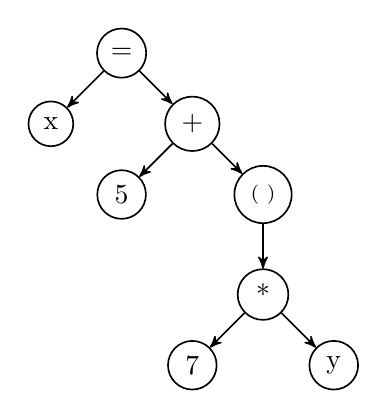
\begin{tikzpicture}[->,>=stealth',auto,
                    node distance=0.5in,semithick]
\tikzstyle{every node}=[draw,circle]
\node (A) {=};
\node (B) [below left of=A] {x};
\node (C) [below right of=A] {+};
\node (D) [below left of=C] {5};
\node (E) [below right of=C] {\scalefont{0.7}(~)};
\node (F) [below of=E] {*};
\node (G) [below left of=F] {7};
\node (H) [below right of=F] {y};

\path (A) edge (B) edge (C)
      (C) edge (D) edge (E)
      (E) edge (F)
      (F) edge (G) edge (H);
\end{tikzpicture}
\end{document}
